%\documentclass[reponses, utf8, 11pt]{feuille}
\documentclass[utf8, 11pt]{feuille}

\newcommand{\titredutd}{\textbf{TD6 --- Deux approches pour l'oscillateur harmonique}}

\begin{document}


\begin{tcolorbox}[
        colback=gray!20,
        colframe=gray!20,
        width=\dimexpr\textwidth\relax, 
        arc=0pt,outer arc=0pt,
        ]

\texttt{Seules les calculatrices non communicantes et les notes manuscrites personnelles sont autorisées.}

\texttt{Les exercices sont totalement indépendants.}

\texttt{On notera $k_B$ la constante de Boltzmann et $h$ la constante de Planck.}

\end{tcolorbox}



% ______________________________________________________________________________
\section{\medium~Le modèle d'Einstein en micro-canonique}

On considère un solide formé de $N$ ions ou atomes vibrant autour de leurs positions d'équilibre avec la même fréquence $\nu$. On suppose que ce solide est isolé thermiquement et que son énergie est $E$ avec une incertitude que l'on négligera. On rappelle que l'énergie de vibration d'un oscillateur harmonique de fréquence $\nu$ suivant un axe est:
$$
\epsilon_k=(k+\frac{1}{2}) h \nu
$$
où $k$ est un entier naturel. Soit $E \gg \frac{3N}{2} h \nu$, l'énergie associée aux vibrations du solide.

\question
Calculer le nombre de micro-états $\Omega(E,N)$ du système.

\question
En déduire l'expression de l'entropie $S(E,N)$.

\question
Déterminer la température $T$ du solide à l'équilibre. 

\question
Inverser la relation précédente et montrer que l'énergie $E$ s'exprime en fonction de $\beta=\frac{1}{k_BT}$ comme
$$
E=\frac{3}{2} N h \nu + \frac{3Nh \nu}{e^{\beta h \nu}-1}. \nonumber
$$

\question
Comment varie l'énergie à haute température ? En déduire la capacité calorifique du solide dans cette limite. Quelle loi bien connue retrouve-t-on ?



% ______________________________________________________________________________
\section{\medium~Système d'oscillateurs harmoniques classiques}

On considère un système constitué de $N \gg 1$ oscillateurs harmoniques {\it classiques}, de masse $m$, de pulsation propre $\omega$, localisés sur un axe à une dimension et {\it indépendants}.

On rappelle que l'énergie mécanique d'un oscillateur harmonique est :
$$
\epsilon=\frac{m}{2}\omega^2 x^2+\frac{p_x^2}{2m} , \nonumber
$$
où $x$ est l'abscisse de l'écart à la position d'équilibre et $p_x$ la quantité de mouvement associée.

\question
Calculer le volume dans l'espace des phases des états d'énergie inférieure ou égale à $E$. Par des changements de variables appropriés, on fera apparaître le volume $V_{2N}$ de la boule de dimension $2N$ de rayon $R=1$, $V_{2N}=\frac{\pi^N}{\Gamma(N+1)}$.

\question
En déduire le nombre de micro-états $\Phi(E,N)$ d'énergie inférieure ou égale à $E$, puis l'entropie $S(E,N)$ du système. L'entropie est-elle bien extensive ?

\question
Calculer la température de ce système, puis sa capacité calorifique. Comparer aux résultats de l'exercice précédent.

\question
Comment généraliser ce résultat pour une collection d'OH 3D ?



% ______________________________________________________________________________
\section{\hard~Question de contact thermique}
En étudiant un système à deux niveaux, nous avons obtenu la température micro-canonique pour les spins nucléaires d'un cristal associée à l'énergie magnétique $E_m$, que nous noterons $T_m(E_m)$. Des inversions de population correspondant à des températures négatives ont été observées dans un cristal de fluorure de lithium. Dans ce système, le temps de relaxation pour l'interaction mutuelle entre les spins nucléaires ($\tau_1 \simeq 10^{-5}$ s) est très court devant le temps de relaxation pour l'interaction entre les spins et le réseau ($\tau_1 \simeq 3 \times 10^{2}$ s). On peut donc rapidement arriver (sur une échelle $\tau_1$) \`a un équilibre thermodynamique du système de spins nucléaires avant que ce système ne se thermalise avec les vibrations du réseau. L'expérience consiste alors à placer le cristal dans un champ magnétique et à renverser très brutalement celui-ci. On est alors, pendant un temps de l'ordre de $\tau_2$ dans un état de température négative (voir figure ci-dessous).

\begin{figure}[!t]
\centering
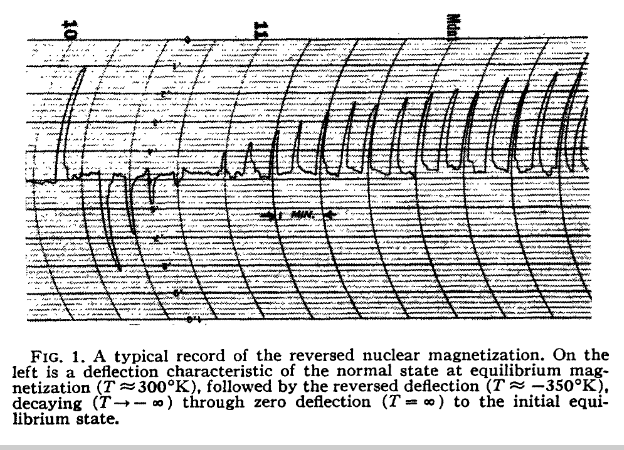
\includegraphics[height=.42 \textwidth]{negative}
\caption{Extrait de l'article : E. M. Purcell and R. V. Pound, Physical Review \textbf{81}, 'A nuclear spin system at negative temperature', p. 279 (1951)}
\label{FTN}
\end{figure}

On considère donc $N$ atomes d'un cristal qui portent chacun un spin-1/2, juste après l'inversion du champ magnétique $B$ qui les avait polarisés. L'énergie magnétique $E_m^i$ est donc positive. Par ailleurs, pour tenir compte les vibrations du cristal, on admet que ces $N$ atomes  portent des oscillateurs harmoniques classiques indépendants 3D (masse $m$, pulsation $\omega$). L'énergie vibrationnelle initiale est notée $E_v^i$.

\question
Rappeler les expressions $S_v(E_v^i,N)$ , $T_v^i$, $S_m(E_m^i,N)$ et $T_m^i$ des entropies et des températures en fonction des données, de $N$, et des énergies initiales.

\question
Mener l'étude du contact thermique entre les degrés de liberté de spins et vibrationnels. Le résultat n'est pas analytique. On déterminera l'équation qui permet de calculer l'énergie magnétique la plus probable, que l'on assimilera à l'énergie magnétique à l'équilibre. Préciser la température d'équilibre $T^f$ que l'on comparera à $T^i_v$ et $T_m^i$.

\question
Décrire thermodynamiquement la transformation du système. Justifier que les températures négatives sont plus chaudes que les températures positives.



\end{document}
